\documentclass[main.tex]{subfiles}

\begin{document}

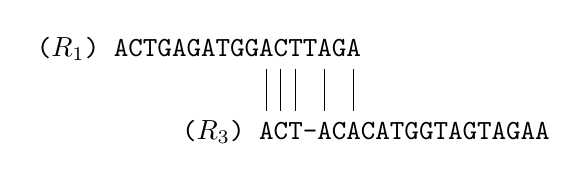
\begin{tikzpicture}[x=0.75pt,y=0.75pt,yscale=-1,xscale=1]
 \draw    (138, 50) -- (138, 70) ;
 \draw    (145, 50) -- (145, 70) ;
 \draw    (152, 50) -- (152, 70) ;
%\draw    (159, 50) -- (159, 70) ;
 \draw    (166, 50) -- (166, 70) ;
%\draw    (173, 50) -- (173, 70) ;
 \draw    (180, 50) -- (180, 70) ;

\draw (105.5,40) node  [align=left] {\texttt{($R_1$) ACTGAGATGGACTTAGA}};
\draw (186,80) node  [align=left] {\texttt{($R_3$) ACT-ACACATGGTAGTAGAA}};

\end{tikzpicture}

\end{document}
